\documentclass[fleqn,11pt,aspectratio=43]{beamer}
\usepackage[utf8x]{inputenc}
\usepackage[T1]{fontenc}
\usepackage[ngerman]{babel}
\usepackage{stmaryrd}
\usepackage{amsfonts}
\usepackage{amssymb}
\usepackage{amsmath}
\usepackage{microtype}

\usepackage{listings}
\usepackage{color}
\usepackage{pxfonts}

\definecolor{mygreen}{RGB}{51,141,120}
\definecolor{myblue}{RGB}{0,128,180}
\definecolor{myviolet}{RGB}{118,0,118}

\lstset{ %
  language=Haskell,
  backgroundcolor=\color{white},         % choose the background color
  basicstyle=\ttfamily\footnotesize,     % size of fonts used for the code
  numbers=none,
  breaklines=true,                       % automatic line breaking only at whitespace
  captionpos=b,                          % sets the caption-position to bottom
  commentstyle=\color{mygreen},    % comment style
  escapeinside={\%*}{*)},                % if you want to add LaTeX within your code
  keywordstyle=\color{myblue}\bfseries, % keyword style
  stringstyle=\color{myviolet},    % string literal style
  frame=single,
  tabsize=2
}
\usepackage{tikz}
\usetikzlibrary{
  arrows,
  shapes.misc,
  shapes.arrows,
  chains,
  matrix,
  positioning,
  scopes,
  decorations.pathmorphing,
  shadows,
  backgrounds
}


\usetheme[%
  %cmyk,%<cmyk/rgbprint>,          Auswahl des Farbmodells
  orange,%<blue/orange/green/violet> Auswahl des Sekundärfarbklangs
  %dark,%<light,medium>        Auswahl der Helligkeit
  %colorhead,%    Farbig hinterlegte Kopfleiste
  %colorfoot,%    Farbig hinterlegt Fußleiste auf Titelseite
  %colorblocks,%   Blöcke Farbig hinterlegen
  %nopagenum,%    Keine Seitennumer in Fußzeile
  %nodate,%       Kein Datum in Fußleiste
  %tocinheader,%   Inhaltsverzeichnis in Kopfleiste
  %tinytocinheader,% kleines Kopfleisten-Inhaltsverzeichnis
  %widetoc,%      breites Kopfleisten-Inhaltsverzeichnis
  %narrowtoc,%    schmales Kopfleisten-Inhaltsverzeichnis
  %nosubsectionsinheader,%  Keine subsections im Kopfleisten-Inhaltsverzeichnis
  %nologoinfoot,% Kein Logo im Fußbereich darstellen
  ]{tubs}

\titlegraphic[scaled]{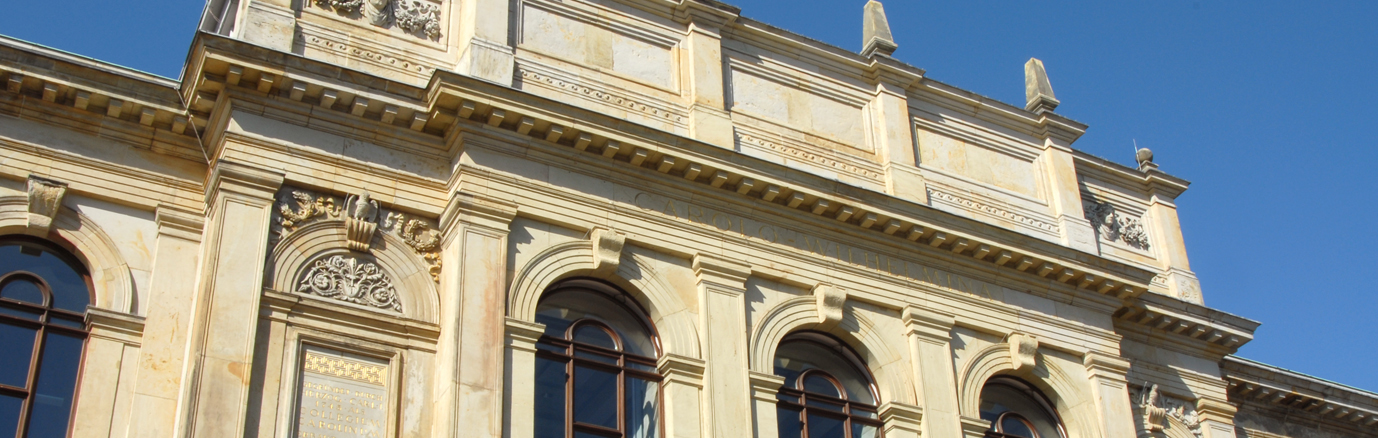
\includegraphics{img/titlepicture.jpg}}
\logo{
\includegraphics{img/logo_mit_text.pdf}}

\AtBeginSection[]{
  \begin{frame}[noframenumbering] 
  		\scriptsize
  		\frametitle{Überblick}  
  		\tableofcontents[currentsection, hideallsubsections]
  \end{frame}
}

\AtBeginSubsection[]{
  \begin{frame}[noframenumbering]
    	\scriptsize 
  		\frametitle{\insertsectionhead - \insertsubsectionhead} 
  		\tableofcontents[ 
  			currentsubsection, 
  		    sectionstyle=show/hide, 
  		   	subsectionstyle=show/shaded/hide] 
  \end{frame}
}


\title{Programmieren für Fortgeschrittene - \\eine Einführung in Haskell}

\author[Stephan Mielke]{\emph{Stephan Mielke}}
\institute[TU Braunschweig, IPS]{Technische Universität Braunschweig, IPS}


\begin{document}

\subtitle{Teil drei - noch etwas mehr} 
\date{15.12.2014}

\begin{frame}[plain, noframenumbering]
\titlepage
\end{frame}

\begin{frame}[noframenumbering]
  \scriptsize
  %\frametitle{\insertsectionhead}  
  \frametitle{Überblick}  
  %\begin{block}{\vspace*{-2ex}}
    \tableofcontents[currentsection,sectionstyle=show, hideallsubsections]
  %end{block} 
\end{frame}

\section{Typkonstruktoren}
\subsection{Eigene Datentypen}
\frame{
\frametitle{Typkonstruktoren - Aufzählungstyp}
\only<1>{
\begin{block}{\vspace*{-3ex}}
Aufzählungstypen sind mit Enums aus C bzw. C++ zu vergleichen und fassen inhaltlich Elemente zusammen
\end{block}
}
\only<1-2>{
\begin{block}{\lstinline|data|}
\begin{center}
\scalebox{0.6}{\begin{tikzpicture}[
      nonterminal/.style={
         rectangle,
         minimum size=5.0mm,
         very thick,
         draw=blue!50!black!50,
         top color=white,
         bottom color=blue!50!black!20,
         font=\itshape\scriptsize,
         %text height=1.5ex,
         %text depth=.25ex
      },
      terminal/.style={
         rounded rectangle,
         minimum size=5.0mm,
         very thick,draw=black!50,
         top color=white,bottom color=black!20,
         font=\ttfamily\scriptsize,
         %text height=1.5ex,
         %text depth=.25ex
      },
      skip loop/.style={
         to path={-- ++(0,#1) -| (\tikztotarget)}
      },
      point/.style={coordinate},>=stealth',thick,draw=black!50,
      tip/.style={->,shorten >=0.007pt},every join/.style={rounded corners},
      hv path/.style={to path={-| (\tikztotarget)}},
      vh path/.style={to path={|- (\tikztotarget)}},
      %text height=1.5ex,text depth=.25ex
    ]
    \matrix[column sep=5.0mm, row sep=3.0mm] {
 &  &  &  &  & \node (n16) [point] {}; &  &  &  &  & \\
\node (n21) [circle, draw, inner sep=0pt, minimum size=0.75ex] {}; & \node (n22) [terminal] {data}; & \node (n23) [nonterminal] {Datentyp}; & \node (n24) [terminal] {=}; & \node (n25) [point] {}; & \node (n26) [nonterminal] {Konstruktor}; & \node (n27) [terminal] {|}; & \node (n28) [point] {}; & \node (n29) [point] {}; &  & \\
 &  &  &  &  &  &  &  &  &  & \\
 &  &  &  &  & \node (n46) [point] {}; &  &  &  &  & \\
 &  &  &  &  & \node (n56) [point] {}; &  &  &  &  & \\
\node (n61) [point] {}; & \node (n62) [point] {}; & \node (n63) [terminal] {deriving}; & \node (n64) [terminal] {(}; & \node (n65) [point] {}; & \node (n66) [nonterminal] {Typklasse}; & \node (n67) [terminal] {,}; & \node (n68) [point] {}; & \node (n69) [terminal] {)}; & \node (n610) [point] {}; & \node (n611) [circle, draw, inner sep=0pt, minimum size=0.75ex] {};\\
    };
  { [start chain]
       \chainin (n21);
       \chainin (n22)    [join=by tip];
  }
  { [start chain]
       \chainin (n22);
       \chainin (n23)    [join=by tip];
  }
  { [start chain]
       \chainin (n23);
       \chainin (n24)    [join=by tip];
  }
  { [start chain]
       \chainin (n24);
       \chainin (n25)    [join];
  }
  { [start chain]
       \chainin (n25);
       \chainin (n26)    [join=by tip];
  }
  { [start chain]
       \chainin (n26);
       \chainin (n27)    [join=by tip];
  }
  { [start chain]
       \chainin (n27);
       \chainin (n28)    [join];
  }
  { [start chain]
       \chainin (n28);
       \chainin (n29)    [join=by tip];
  }
  { [start chain]
       \chainin (n61);
       \chainin (n62)    [join];
  }
  { [start chain]
       \chainin (n62);
       \chainin (n63)    [join=by tip];
  }
  { [start chain]
       \chainin (n63);
       \chainin (n64)    [join=by tip];
  }
  { [start chain]
       \chainin (n64);
       \chainin (n65)    [join];
  }
  { [start chain]
       \chainin (n65);
       \chainin (n66)    [join=by tip];
  }
  { [start chain]
       \chainin (n66);
       \chainin (n67)    [join=by tip];
  }
  { [start chain]
       \chainin (n67);
       \chainin (n68)    [join];
  }
  { [start chain]
       \chainin (n68);
       \chainin (n69)    [join=by tip];
  }
  { [start chain]
       \chainin (n69);
       \chainin (n610)    [join];
  }
  { [start chain]
       \chainin (n610);
       \chainin (n611)    [join=by tip];
  }
  { [start chain]
       \chainin (n28);
       \chainin (n16)    [join=by vh path];
       \chainin (n25)    [join=by {hv path,tip}];
  }
  { [start chain]
       \chainin (n68);
       \chainin (n56)    [join=by vh path];
       \chainin (n65)    [join=by {hv path,tip}];
  }
  { [start chain]
       \chainin (n62);
       \chainin (n46)    [join=by vh path];
       \chainin (n610)    [join=by {hv path,tip}];
  }
\end{tikzpicture}
}
\end{center}
\end{block}}
\only<2>{
\begin{block}{Konstruktor}
\begin{center}
\scalebox{0.6}{\begin{tikzpicture}[
      nonterminal/.style={
         rectangle,
         minimum size=5.0mm,
         very thick,
         draw=blue!50!black!50,
         top color=white,
         bottom color=blue!50!black!20,
         font=\itshape\scriptsize,
         %text height=1.5ex,
         %text depth=.25ex
      },
      terminal/.style={
         rounded rectangle,
         minimum size=5.0mm,
         very thick,draw=black!50,
         top color=white,bottom color=black!20,
         font=\ttfamily\scriptsize,
         %text height=1.5ex,
         %text depth=.25ex
      },
      skip loop/.style={
         to path={-- ++(0,#1) -| (\tikztotarget)}
      },
      point/.style={coordinate},>=stealth',thick,draw=black!50,
      tip/.style={->,shorten >=0.007pt},every join/.style={rounded corners},
      hv path/.style={to path={-| (\tikztotarget)}},
      vh path/.style={to path={|- (\tikztotarget)}},
      %text height=1.5ex,text depth=.25ex
    ]
    \matrix[column sep=5.0mm, row sep=3.0mm] {
 &  &  &  & \node (n15) [terminal] {->}; & \node (n16) [nonterminal] {AttrTyp}; &  &  & \\
\node (n21) [circle, draw, inner sep=0pt, minimum size=0.75ex] {}; & \node (n22) [nonterminal] {Konstruktor}; & \node (n23) [terminal] {::}; & \node (n24) [point] {}; &  &  & \node (n27) [point] {}; & \node (n28) [nonterminal] {Datentyp}; & \node (n29) [circle, draw, inner sep=0pt, minimum size=0.75ex] {};\\
    };
  { [start chain]
       \chainin (n21);
       \chainin (n22)    [join=by tip];
  }
  { [start chain]
       \chainin (n22);
       \chainin (n23)    [join=by tip];
  }
  { [start chain]
       \chainin (n23);
       \chainin (n24)    [join];
  }
  { [start chain]
       \chainin (n24);
       \chainin (n27)    [join];
  }
  { [start chain]
       \chainin (n15);
       \chainin (n16)    [join=by tip];
  }
  { [start chain]
       \chainin (n27);
       \chainin (n16)    [join=by {vh path,tip}];
  }
  { [start chain]
       \chainin (n15);
       \chainin (n24)    [join=by {hv path,tip}];
  }
  { [start chain]
       \chainin (n27);
       \chainin (n28)    [join=by tip];
  }
  { [start chain]
       \chainin (n28);
       \chainin (n29)    [join=by tip];
  }
\end{tikzpicture}
}
\end{center}
In diesem Fall erhält der Konstruktor keine Parameter.
\end{block}
}
}

\begin{frame}[fragile]
\frametitle{Typkonstruktoren - Aufzählungstyp} 
\begin{block}{\vspace*{-3ex}}
\lstinline!data Color = Blue | Cyan | Yellow | Orange | Green!
\end{block}
\pause
\only<2>{Wie werden die Konstuktoren aussehen ?}
\pause
Konstruktoren:
\begin{lstlisting}
Blue   :: Color
Cyan   :: Color
Yellow :: Color
Orange :: Color
Green  :: Color
\end{lstlisting}
\end{frame}

\frame{
\frametitle{Typkonstruktoren - Produkttyp}
\only<1>{
\begin{block}{\vspace*{-3ex}}
\begin{itemize}
  \item Produkttyp ist ein Tupel der einzelnen Attribute
  \item Tupel fassen Gruppen von Daten zusammen, die logisch zusammen gehören und gemeinsam etwas Neues und Eigenständiges bilden
\end{itemize}
\end{block}
}

\only<1-3>{
\begin{block}{\lstinline|data| mit allen Angaben}
\begin{center}
\scalebox{0.6}{\begin{tikzpicture}[
      nonterminal/.style={
         rectangle,
         minimum size=5.0mm,
         very thick,
         draw=blue!50!black!50,
         top color=white,
         bottom color=blue!50!black!20,
         font=\itshape\scriptsize,
         %text height=1.5ex,
         %text depth=.25ex
      },
      terminal/.style={
         rounded rectangle,
         minimum size=5.0mm,
         very thick,draw=black!50,
         top color=white,bottom color=black!20,
         font=\ttfamily\scriptsize,
         %text height=1.5ex,
         %text depth=.25ex
      },
      skip loop/.style={
         to path={-- ++(0,#1) -| (\tikztotarget)}
      },
      point/.style={coordinate},>=stealth',thick,draw=black!50,
      tip/.style={->,shorten >=0.007pt},every join/.style={rounded corners},
      hv path/.style={to path={-| (\tikztotarget)}},
      vh path/.style={to path={|- (\tikztotarget)}},
      %text height=1.5ex,text depth=.25ex
    ]
    \matrix[column sep=5.0mm, row sep=3.0mm] {
 &  &  &  &  &  &  &  & \node (n19) [point] {}; &  &  &  & \\
\node (n21) [circle, draw, inner sep=0pt, minimum size=0.75ex] {}; & \node (n22) [terminal] {data}; & \node (n23) [nonterminal] {Datentyp}; & \node (n24) [terminal] {=}; & \node (n25) [nonterminal] {Konstruktor}; & \node (n26) [terminal] {\{}; & \node (n27) [point] {}; & \node (n28) [nonterminal] {Attributname}; & \node (n29) [terminal] {::}; & \node (n210) [nonterminal] {Typ}; & \node (n211) [point] {}; & \node (n212) [terminal] {\}}; & \node (n213) [point] {};\\
 &  &  &  &  &  &  &  &  &  &  &  & \\
 &  &  &  &  & \node (n46) [point] {}; &  &  &  &  &  &  & \\
 &  &  &  &  & \node (n56) [point] {}; &  &  &  &  &  &  & \\
\node (n61) [point] {}; & \node (n62) [point] {}; & \node (n63) [terminal] {deriving}; & \node (n64) [terminal] {(}; & \node (n65) [point] {}; & \node (n66) [nonterminal] {Typklasse}; & \node (n67) [terminal] {,}; & \node (n68) [point] {}; & \node (n69) [terminal] {)}; & \node (n610) [point] {}; & \node (n611) [circle, draw, inner sep=0pt, minimum size=0.75ex] {}; &  & \\
    };
  { [start chain]
       \chainin (n21);
       \chainin (n22)    [join=by tip];
  }
  { [start chain]
       \chainin (n22);
       \chainin (n23)    [join=by tip];
  }
  { [start chain]
       \chainin (n23);
       \chainin (n24)    [join=by tip];
  }
  { [start chain]
       \chainin (n24);
       \chainin (n25)    [join=by tip];
  }
  { [start chain]
       \chainin (n25);
       \chainin (n26)    [join=by tip];
  }
  { [start chain]
       \chainin (n26);
       \chainin (n27)    [join];
  }
  { [start chain]
       \chainin (n27);
       \chainin (n28)    [join=by tip];
  }
  { [start chain]
       \chainin (n28);
       \chainin (n29)    [join=by tip];
  }
  { [start chain]
       \chainin (n29);
       \chainin (n210)    [join=by tip];
  }
  { [start chain]
       \chainin (n210);
       \chainin (n211)    [join];
  }
  { [start chain]
       \chainin (n211);
       \chainin (n212)    [join=by tip];
  }
  { [start chain]
       \chainin (n212);
       \chainin (n213)    [join=by tip];
  }
  { [start chain]
       \chainin (n61);
       \chainin (n62)    [join];
  }
  { [start chain]
       \chainin (n62);
       \chainin (n63)    [join=by tip];
  }
  { [start chain]
       \chainin (n63);
       \chainin (n64)    [join=by tip];
  }
  { [start chain]
       \chainin (n64);
       \chainin (n65)    [join];
  }
  { [start chain]
       \chainin (n65);
       \chainin (n66)    [join=by tip];
  }
  { [start chain]
       \chainin (n66);
       \chainin (n67)    [join=by tip];
  }
  { [start chain]
       \chainin (n67);
       \chainin (n68)    [join];
  }
  { [start chain]
       \chainin (n68);
       \chainin (n69)    [join=by tip];
  }
  { [start chain]
       \chainin (n69);
       \chainin (n610)    [join];
  }
  { [start chain]
       \chainin (n610);
       \chainin (n611)    [join=by tip];
  }
  { [start chain]
       \chainin (n211);
       \chainin (n19)    [join=by vh path];
       \chainin (n27)    [join=by {hv path,tip}];
  }
  { [start chain]
       \chainin (n68);
       \chainin (n56)    [join=by vh path];
       \chainin (n65)    [join=by {hv path,tip}];
  }
  { [start chain]
       \chainin (n62);
       \chainin (n46)    [join=by vh path];
       \chainin (n610)    [join=by {hv path,tip}];
  }
\end{tikzpicture}
}
\end{center}
\end{block}}
\only<2>{
\begin{block}{Konstruktor}
\begin{center}
\scalebox{0.6}{\begin{tikzpicture}[
      nonterminal/.style={
         rectangle,
         minimum size=5.0mm,
         very thick,
         draw=blue!50!black!50,
         top color=white,
         bottom color=blue!50!black!20,
         font=\itshape\scriptsize,
         %text height=1.5ex,
         %text depth=.25ex
      },
      terminal/.style={
         rounded rectangle,
         minimum size=5.0mm,
         very thick,draw=black!50,
         top color=white,bottom color=black!20,
         font=\ttfamily\scriptsize,
         %text height=1.5ex,
         %text depth=.25ex
      },
      skip loop/.style={
         to path={-- ++(0,#1) -| (\tikztotarget)}
      },
      point/.style={coordinate},>=stealth',thick,draw=black!50,
      tip/.style={->,shorten >=0.007pt},every join/.style={rounded corners},
      hv path/.style={to path={-| (\tikztotarget)}},
      vh path/.style={to path={|- (\tikztotarget)}},
      %text height=1.5ex,text depth=.25ex
    ]
    \matrix[column sep=5.0mm, row sep=3.0mm] {
 &  &  &  & \node (n15) [terminal] {->}; & \node (n16) [nonterminal] {AttrTyp}; &  &  & \\
\node (n21) [circle, draw, inner sep=0pt, minimum size=0.75ex] {}; & \node (n22) [nonterminal] {Konstruktor}; & \node (n23) [terminal] {::}; & \node (n24) [point] {}; &  &  & \node (n27) [point] {}; & \node (n28) [nonterminal] {Datentyp}; & \node (n29) [circle, draw, inner sep=0pt, minimum size=0.75ex] {};\\
    };
  { [start chain]
       \chainin (n21);
       \chainin (n22)    [join=by tip];
  }
  { [start chain]
       \chainin (n22);
       \chainin (n23)    [join=by tip];
  }
  { [start chain]
       \chainin (n23);
       \chainin (n24)    [join];
  }
  { [start chain]
       \chainin (n24);
       \chainin (n27)    [join];
  }
  { [start chain]
       \chainin (n15);
       \chainin (n16)    [join=by tip];
  }
  { [start chain]
       \chainin (n27);
       \chainin (n16)    [join=by {vh path,tip}];
  }
  { [start chain]
       \chainin (n15);
       \chainin (n24)    [join=by {hv path,tip}];
  }
  { [start chain]
       \chainin (n27);
       \chainin (n28)    [join=by tip];
  }
  { [start chain]
       \chainin (n28);
       \chainin (n29)    [join=by tip];
  }
\end{tikzpicture}
}
\end{center}
\end{block}}
\only<3>{
\begin{block}{Selektor (bei allen Angaben automatisch erstellt)}
\begin{center}
\scalebox{0.6}{\begin{tikzpicture}[
      nonterminal/.style={
         rectangle,
         minimum size=5.0mm,
         very thick,
         draw=blue!50!black!50,
         top color=white,
         bottom color=blue!50!black!20,
         font=\itshape\scriptsize,
         %text height=1.5ex,
         %text depth=.25ex
      },
      terminal/.style={
         rounded rectangle,
         minimum size=5.0mm,
         very thick,draw=black!50,
         top color=white,bottom color=black!20,
         font=\ttfamily\scriptsize,
         %text height=1.5ex,
         %text depth=.25ex
      },
      skip loop/.style={
         to path={-- ++(0,#1) -| (\tikztotarget)}
      },
      point/.style={coordinate},>=stealth',thick,draw=black!50,
      tip/.style={->,shorten >=0.007pt},every join/.style={rounded corners},
      hv path/.style={to path={-| (\tikztotarget)}},
      vh path/.style={to path={|- (\tikztotarget)}},
      %text height=1.5ex,text depth=.25ex
    ]
    \matrix[column sep=5.0mm, row sep=3.0mm] {
\node (n11) [circle, draw, inner sep=0pt, minimum size=0.75ex] {}; & \node (n12) [nonterminal] {Attributname}; & \node (n13) [terminal] {::}; & \node (n14) [nonterminal] {Datentyp}; & \node (n15) [terminal] {->}; & \node (n16) [nonterminal] {AttrTyp}; & \node (n17) [circle, draw, inner sep=0pt, minimum size=0.75ex] {};\\
    };
  { [start chain]
       \chainin (n11);
       \chainin (n12)    [join=by tip];
  }
  { [start chain]
       \chainin (n12);
       \chainin (n13)    [join=by tip];
  }
  { [start chain]
       \chainin (n13);
       \chainin (n14)    [join=by tip];
  }
  { [start chain]
       \chainin (n14);
       \chainin (n15)    [join=by tip];
  }
  { [start chain]
       \chainin (n15);
       \chainin (n16)    [join=by tip];
  }
  { [start chain]
       \chainin (n16);
       \chainin (n17)    [join=by tip];
  }
\end{tikzpicture}
}
\end{center}
\end{block}}
}

\begin{frame}[fragile]
\frametitle{Typkonstruktoren - Produkttyp} 
\begin{block}{\vspace*{-3ex}}
\lstinline|data Point = Point{x :: Double, y :: Double}|
\end{block}
\only<2>{
\begin{block}{Kurz}
\lstinline|data Point = Point Double Double|
\end{block}
\vspace*{-1ex}
}

\begin{block}{\vspace*{-3ex}}
\lstinline|data Circle = Circle{center :: Point, radius :: Double}|
\end{block}
\only<2>{
\begin{block}{Kurz}
\lstinline|data Circle = Circle Point Double|
\end{block}
}

\only<2>{\begin{alertblock}{Kurz Schreibweise}
Bei der kurz Schreibweise werden keine Selektoren erstellt
\end{alertblock}}
\end{frame}

\begin{frame}[fragile]
\frametitle{Typkonstruktoren - Produkttyp}
\begin{block}{\vspace*{-3ex}}
\lstinline|data Point = Point{x :: Double, y :: Double}|
\lstinline|data Circle = Circle{center :: Point, radius :: Double}|
\end{block} 
Konstruktorfunktionen: 
\only<1>{?}\pause
\begin{lstlisting}
Point :: Double -> Double -> Point
Circle :: Point -> Double -> Circle
\end{lstlisting}
\end{frame}

\begin{frame}[fragile]
\frametitle{Typkonstruktoren - Produkttyp} 
\begin{block}{\vspace*{-3ex}}
\lstinline|data Point = Point{x :: Double, y :: Double}|
\lstinline|data Circle = Circle{center :: Point, radius :: Double}|
\end{block} 
Selektorfunktionen: 
\only<1>{?}\pause
\begin{lstlisting}
x :: Point -> Double
y :: Point -> Double
center :: Circle -> Point
radius :: Circle -> Double
\end{lstlisting}
\end{frame}

\frame{\frametitle{Typkonstruktoren - Summentyp}
\only<1>{
\begin{block}{\vspace*{-3ex}}
\begin{itemize}
\item Summentypen fassen inhaltlich verwandte (aber struktuell verschiedene) Elemente zusammen
\item Sind eine Fusion von Aufzählungs- und Produkttyp
\end{itemize}
\end{block}
}
\only<1-3>{
\begin{block}{\lstinline|data| mit allen Angaben}
\begin{center}
\scalebox{0.6}{\begin{tikzpicture}[
      nonterminal/.style={
         rectangle,
         minimum size=5.0mm,
         very thick,
         draw=blue!50!black!50,
         top color=white,
         bottom color=blue!50!black!20,
         font=\itshape\scriptsize,
         %text height=1.5ex,
         %text depth=.25ex
      },
      terminal/.style={
         rounded rectangle,
         minimum size=5.0mm,
         very thick,draw=black!50,
         top color=white,bottom color=black!20,
         font=\ttfamily\scriptsize,
         %text height=1.5ex,
         %text depth=.25ex
      },
      skip loop/.style={
         to path={-- ++(0,#1) -| (\tikztotarget)}
      },
      point/.style={coordinate},>=stealth',thick,draw=black!50,
      tip/.style={->,shorten >=0.007pt},every join/.style={rounded corners},
      hv path/.style={to path={-| (\tikztotarget)}},
      vh path/.style={to path={|- (\tikztotarget)}},
      %text height=1.5ex,text depth=.25ex
    ]
    \matrix[column sep=5.0mm, row sep=3.0mm] {
 &  &  &  &  &  &  &  &  & \node (n110) [point] {}; &  &  &  &  &  & \\
 &  &  &  &  &  &  &  &  & \node (n210) [point] {}; &  &  &  &  &  & \\
\node (n31) [circle, draw, inner sep=0pt, minimum size=0.75ex] {}; & \node (n32) [terminal] {data}; & \node (n33) [nonterminal] {Datentyp}; & \node (n34) [terminal] {=}; & \node (n35) [point] {}; & \node (n36) [nonterminal] {Konstruktor}; & \node (n37) [terminal] {\{}; & \node (n38) [point] {}; & \node (n39) [nonterminal] {Attributname}; & \node (n310) [terminal] {::}; & \node (n311) [nonterminal] {Typ}; & \node (n312) [point] {}; & \node (n313) [terminal] {\}}; & \node (n314) [terminal] {|}; & \node (n315) [point] {}; & \node (n316) [point] {};\\
 &  &  &  &  &  &  &  &  &  &  &  &  &  &  & \\
 &  &  &  &  & \node (n56) [point] {}; &  &  &  &  &  &  &  &  &  & \\
 &  &  &  &  & \node (n66) [point] {}; &  &  &  &  &  &  &  &  &  & \\
\node (n71) [point] {}; & \node (n72) [point] {}; & \node (n73) [terminal] {deriving}; & \node (n74) [terminal] {(}; & \node (n75) [point] {}; & \node (n76) [nonterminal] {Typklasse}; & \node (n77) [terminal] {,}; & \node (n78) [point] {}; & \node (n79) [terminal] {)}; & \node (n710) [point] {}; & \node (n711) [circle, draw, inner sep=0pt, minimum size=0.75ex] {}; &  &  &  &  & \\
    };
  { [start chain]
       \chainin (n31);
       \chainin (n32)    [join=by tip];
  }
  { [start chain]
       \chainin (n32);
       \chainin (n33)    [join=by tip];
  }
  { [start chain]
       \chainin (n33);
       \chainin (n34)    [join=by tip];
  }
  { [start chain]
       \chainin (n34);
       \chainin (n35)    [join];
  }
  { [start chain]
       \chainin (n35);
       \chainin (n36)    [join=by tip];
  }
  { [start chain]
       \chainin (n36);
       \chainin (n37)    [join=by tip];
  }
  { [start chain]
       \chainin (n37);
       \chainin (n38)    [join];
  }
  { [start chain]
       \chainin (n38);
       \chainin (n39)    [join=by tip];
  }
  { [start chain]
       \chainin (n39);
       \chainin (n310)    [join=by tip];
  }
  { [start chain]
       \chainin (n310);
       \chainin (n311)    [join=by tip];
  }
  { [start chain]
       \chainin (n311);
       \chainin (n312)    [join];
  }
  { [start chain]
       \chainin (n312);
       \chainin (n313)    [join=by tip];
  }
  { [start chain]
       \chainin (n313);
       \chainin (n314)    [join=by tip];
  }
  { [start chain]
       \chainin (n314);
       \chainin (n315)    [join];
  }
  { [start chain]
       \chainin (n315);
       \chainin (n316)    [join=by tip];
  }
  { [start chain]
       \chainin (n71);
       \chainin (n72)    [join];
  }
  { [start chain]
       \chainin (n72);
       \chainin (n73)    [join=by tip];
  }
  { [start chain]
       \chainin (n73);
       \chainin (n74)    [join=by tip];
  }
  { [start chain]
       \chainin (n74);
       \chainin (n75)    [join];
  }
  { [start chain]
       \chainin (n75);
       \chainin (n76)    [join=by tip];
  }
  { [start chain]
       \chainin (n76);
       \chainin (n77)    [join=by tip];
  }
  { [start chain]
       \chainin (n77);
       \chainin (n78)    [join];
  }
  { [start chain]
       \chainin (n78);
       \chainin (n79)    [join=by tip];
  }
  { [start chain]
       \chainin (n79);
       \chainin (n710)    [join];
  }
  { [start chain]
       \chainin (n710);
       \chainin (n711)    [join=by tip];
  }
  { [start chain]
       \chainin (n312);
       \chainin (n210)    [join=by vh path];
       \chainin (n38)    [join=by {hv path,tip}];
  }
  { [start chain]
       \chainin (n315);
       \chainin (n110)    [join=by vh path];
       \chainin (n35)    [join=by {hv path,tip}];
  }
  { [start chain]
       \chainin (n78);
       \chainin (n66)    [join=by vh path];
       \chainin (n75)    [join=by {hv path,tip}];
  }
  { [start chain]
       \chainin (n72);
       \chainin (n56)    [join=by vh path];
       \chainin (n710)    [join=by {hv path,tip}];
  }
\end{tikzpicture}
}
\end{center}
\end{block}}
\only<2>{
\begin{block}{Konstruktor}
\begin{center}
\scalebox{0.6}{\begin{tikzpicture}[
      nonterminal/.style={
         rectangle,
         minimum size=5.0mm,
         very thick,
         draw=blue!50!black!50,
         top color=white,
         bottom color=blue!50!black!20,
         font=\itshape\scriptsize,
         %text height=1.5ex,
         %text depth=.25ex
      },
      terminal/.style={
         rounded rectangle,
         minimum size=5.0mm,
         very thick,draw=black!50,
         top color=white,bottom color=black!20,
         font=\ttfamily\scriptsize,
         %text height=1.5ex,
         %text depth=.25ex
      },
      skip loop/.style={
         to path={-- ++(0,#1) -| (\tikztotarget)}
      },
      point/.style={coordinate},>=stealth',thick,draw=black!50,
      tip/.style={->,shorten >=0.007pt},every join/.style={rounded corners},
      hv path/.style={to path={-| (\tikztotarget)}},
      vh path/.style={to path={|- (\tikztotarget)}},
      %text height=1.5ex,text depth=.25ex
    ]
    \matrix[column sep=5.0mm, row sep=3.0mm] {
 &  &  &  & \node (n15) [terminal] {->}; & \node (n16) [nonterminal] {AttrTyp}; &  &  & \\
\node (n21) [circle, draw, inner sep=0pt, minimum size=0.75ex] {}; & \node (n22) [nonterminal] {Konstruktor}; & \node (n23) [terminal] {::}; & \node (n24) [point] {}; &  &  & \node (n27) [point] {}; & \node (n28) [nonterminal] {Datentyp}; & \node (n29) [circle, draw, inner sep=0pt, minimum size=0.75ex] {};\\
    };
  { [start chain]
       \chainin (n21);
       \chainin (n22)    [join=by tip];
  }
  { [start chain]
       \chainin (n22);
       \chainin (n23)    [join=by tip];
  }
  { [start chain]
       \chainin (n23);
       \chainin (n24)    [join];
  }
  { [start chain]
       \chainin (n24);
       \chainin (n27)    [join];
  }
  { [start chain]
       \chainin (n15);
       \chainin (n16)    [join=by tip];
  }
  { [start chain]
       \chainin (n27);
       \chainin (n16)    [join=by {vh path,tip}];
  }
  { [start chain]
       \chainin (n15);
       \chainin (n24)    [join=by {hv path,tip}];
  }
  { [start chain]
       \chainin (n27);
       \chainin (n28)    [join=by tip];
  }
  { [start chain]
       \chainin (n28);
       \chainin (n29)    [join=by tip];
  }
\end{tikzpicture}
}
\end{center}
\end{block}}
\only<3>{
\begin{block}{Selektor (bei allen Angaben automatisch erstellt)}
\begin{center}
\scalebox{0.6}{\begin{tikzpicture}[
      nonterminal/.style={
         rectangle,
         minimum size=5.0mm,
         very thick,
         draw=blue!50!black!50,
         top color=white,
         bottom color=blue!50!black!20,
         font=\itshape\scriptsize,
         %text height=1.5ex,
         %text depth=.25ex
      },
      terminal/.style={
         rounded rectangle,
         minimum size=5.0mm,
         very thick,draw=black!50,
         top color=white,bottom color=black!20,
         font=\ttfamily\scriptsize,
         %text height=1.5ex,
         %text depth=.25ex
      },
      skip loop/.style={
         to path={-- ++(0,#1) -| (\tikztotarget)}
      },
      point/.style={coordinate},>=stealth',thick,draw=black!50,
      tip/.style={->,shorten >=0.007pt},every join/.style={rounded corners},
      hv path/.style={to path={-| (\tikztotarget)}},
      vh path/.style={to path={|- (\tikztotarget)}},
      %text height=1.5ex,text depth=.25ex
    ]
    \matrix[column sep=5.0mm, row sep=3.0mm] {
\node (n11) [circle, draw, inner sep=0pt, minimum size=0.75ex] {}; & \node (n12) [nonterminal] {Attributname}; & \node (n13) [terminal] {::}; & \node (n14) [nonterminal] {Datentyp}; & \node (n15) [terminal] {->}; & \node (n16) [nonterminal] {AttrTyp}; & \node (n17) [circle, draw, inner sep=0pt, minimum size=0.75ex] {};\\
    };
  { [start chain]
       \chainin (n11);
       \chainin (n12)    [join=by tip];
  }
  { [start chain]
       \chainin (n12);
       \chainin (n13)    [join=by tip];
  }
  { [start chain]
       \chainin (n13);
       \chainin (n14)    [join=by tip];
  }
  { [start chain]
       \chainin (n14);
       \chainin (n15)    [join=by tip];
  }
  { [start chain]
       \chainin (n15);
       \chainin (n16)    [join=by tip];
  }
  { [start chain]
       \chainin (n16);
       \chainin (n17)    [join=by tip];
  }
\end{tikzpicture}
}
\end{center}
\end{block}}
}

\begin{frame}[fragile]
\frametitle{Typkonstruktoren - Summentyp} 
\begin{lstlisting}
data Point = Point{x :: Double, y :: Double}

data Shape = Circle{center :: Point, 
    radius :: Double}
  | Rectangle{point :: Point, width :: Double, 
    height :: Double}
  | Triangle{point1 :: Point, point2 :: Point, 
    point3 :: Point}
\end{lstlisting}

\begin{alertblock}{Frage}
Was sind hier Selektoren und Konstruktoren?
\end{alertblock}
\end{frame}

\begin{frame}[fragile]
\frametitle{Typkonstruktoren - Summentyp} 
\begin{lstlisting}
data Shape = Circle{center :: Point, radius :: Double}
  | Rectangle{point :: Point, width :: Double, 
    height :: Double}
  | Triangle{point1 :: Point, point2 :: Point, 
    point3 :: Point}
\end{lstlisting}
Konstruktoren: \only<1>{?}\pause
\begin{lstlisting}
Circle :: Point -> Double -> Shape
Rectangle :: Point -> Double -> Double -> Shape
Triangle :: Point -> Point -> Point -> Shape
\end{lstlisting}
\end{frame}

\begin{frame}[fragile]
\frametitle{Typkonstruktoren - Summentyp}
\begin{lstlisting}
data Shape = Circle{center :: Point, radius :: Double}
  | Rectangle{point :: Point, width :: Double, 
    height :: Double}
  | Triangle{point1 :: Point, point2 :: Point, 
    point3 :: Point}
\end{lstlisting} 
Selektoren: \only<1>{?}\pause
\begin{lstlisting}
center :: Shape -> Point
radius :: Shape -> Double
point :: Shape -> Point
width :: Shape -> Double
...
\end{lstlisting}
\end{frame}
\subsection{Typ-Synonyme}
\frame{\frametitle{Typ-Synonyme}
\begin{block}{\vspace*{-3ex}}
\begin{itemize}
  \item Typ-Synonyme sind keine eigenen Typen sondern führen nur neue Namen für bekannte Typen ein
  \item Vorteile:
    \begin{itemize}
      \item Verbesserte Lesbarkeit
      \item Intern wird bei \lstinline|type Euro = Int| wieder \lstinline|Int|
    \end{itemize}
\end{itemize}
\end{block}
\begin{block}{\vspace*{-3ex}}
\begin{center}
\scalebox{0.8}{\begin{tikzpicture}[
      nonterminal/.style={
         rectangle,
         minimum size=5.0mm,
         very thick,
         draw=blue!50!black!50,
         top color=white,
         bottom color=blue!50!black!20,
         font=\itshape\scriptsize,
         %text height=1.5ex,
         %text depth=.25ex
      },
      terminal/.style={
         rounded rectangle,
         minimum size=5.0mm,
         very thick,draw=black!50,
         top color=white,bottom color=black!20,
         font=\ttfamily\scriptsize,
         %text height=1.5ex,
         %text depth=.25ex
      },
      skip loop/.style={
         to path={-- ++(0,#1) -| (\tikztotarget)}
      },
      point/.style={coordinate},>=stealth',thick,draw=black!50,
      tip/.style={->,shorten >=0.007pt},every join/.style={rounded corners},
      hv path/.style={to path={-| (\tikztotarget)}},
      vh path/.style={to path={|- (\tikztotarget)}},
      %text height=1.5ex,text depth=.25ex
    ]
    \matrix[column sep=5.0mm, row sep=3.0mm] {
\node (n11) [circle, draw, inner sep=0pt, minimum size=0.75ex] {}; & \node (n12) [terminal] {type}; & \node (n13) [nonterminal] {Name}; & \node (n14) [terminal] {=}; & \node (n15) [nonterminal] {bekannter Typ}; & \node (n16) [circle, draw, inner sep=0pt, minimum size=0.75ex] {};\\
    };
  { [start chain]
       \chainin (n11);
       \chainin (n12)    [join=by tip];
  }
  { [start chain]
       \chainin (n12);
       \chainin (n13)    [join=by tip];
  }
  { [start chain]
       \chainin (n13);
       \chainin (n14)    [join=by tip];
  }
  { [start chain]
       \chainin (n14);
       \chainin (n15)    [join=by tip];
  }
  { [start chain]
       \chainin (n15);
       \chainin (n16)    [join=by tip];
  }
\end{tikzpicture}
}
\end{center}
\end{block}
}

\begin{frame}[fragile]
\frametitle{Typ-Synonyme} 
\begin{lstlisting}
type Euro = Int
type Cent = Int
type Preis = (Euro, Cent)

type Tupel = (Int, Int)
\end{lstlisting}
\begin{alertblock}{Achtung}
\lstinline|Preis| und \lstinline|Tupel| sind für uns und intern \lstinline|(Int, Int)|
\end{alertblock}
\end{frame}

\begin{frame}[fragile]
\frametitle{Typ-Synonyme} 
\begin{lstlisting}
type Euro = Int
type Cent = Int

add :: Euro -> Euro -> Euro
add a b = a + b

add' :: Euro -> Cent -> Int
add' a b = a + b
\end{lstlisting}
\begin{alertblock}{Achtung}
\lstinline|add' 5 (add 5 8)| funktioniert
\end{alertblock}
\end{frame}

\begin{frame}[fragile]
\frametitle{Typ-Synonyme mit Typsicherheit} 
\begin{block}{\vspace*{-3ex}}
\begin{itemize}
\item \lstinline|newtype| wird statt \lstinline|type| verwendet, wenn Typsicherheit benötigt wird
\item \lstinline|newtype| verhält sich somit geauso wie \lstinline|data|
\item Jedes \lstinline|newtype| kann durch \lstinline|data| ersetzt werden
\item Jedoch \lstinline|data| kann nur in Ausnahmefällen durch \lstinline|newtype| ersetzt werden
\end{itemize}
\end{block}
\only<1>{
\begin{block}{\vspace*{-3ex}}
\begin{center}
\scalebox{0.8}{\begin{tikzpicture}[
      nonterminal/.style={
         rectangle,
         minimum size=5.0mm,
         very thick,
         draw=blue!50!black!50,
         top color=white,
         bottom color=blue!50!black!20,
         font=\itshape\scriptsize,
         %text height=1.5ex,
         %text depth=.25ex
      },
      terminal/.style={
         rounded rectangle,
         minimum size=5.0mm,
         very thick,draw=black!50,
         top color=white,bottom color=black!20,
         font=\ttfamily\scriptsize,
         %text height=1.5ex,
         %text depth=.25ex
      },
      skip loop/.style={
         to path={-- ++(0,#1) -| (\tikztotarget)}
      },
      point/.style={coordinate},>=stealth',thick,draw=black!50,
      tip/.style={->,shorten >=0.007pt},every join/.style={rounded corners},
      hv path/.style={to path={-| (\tikztotarget)}},
      vh path/.style={to path={|- (\tikztotarget)}},
      %text height=1.5ex,text depth=.25ex
    ]
    \matrix[column sep=5.0mm, row sep=3.0mm] {
\node (n11) [circle, draw, inner sep=0pt, minimum size=0.75ex] {}; & \node (n12) [terminal] {newtype}; & \node (n13) [nonterminal] {Name}; & \node (n14) [terminal] {=}; & \node (n15) [nonterminal] {Name}; & \node (n16) [nonterminal] {bekannter Typ}; & \node (n17) [circle, draw, inner sep=0pt, minimum size=0.75ex] {};\\
    };
  { [start chain]
       \chainin (n11);
       \chainin (n12)    [join=by tip];
  }
  { [start chain]
       \chainin (n12);
       \chainin (n13)    [join=by tip];
  }
  { [start chain]
       \chainin (n13);
       \chainin (n14)    [join=by tip];
  }
  { [start chain]
       \chainin (n14);
       \chainin (n15)    [join=by tip];
  }
  { [start chain]
       \chainin (n15);
       \chainin (n16)    [join=by tip];
  }
  { [start chain]
       \chainin (n16);
       \chainin (n17)    [join=by tip];
  }
\end{tikzpicture}
}
\end{center}
\end{block}
}\pause
\begin{lstlisting}
newtype Euro = Euro Int
newtype Cent = Cent Int
\end{lstlisting}
\begin{alertblock}{Achtung}
\lstinline|Euro| und \lstinline|Cent| sind nicht kompatibel
\end{alertblock}
\end{frame}

\subsection{Rekursive Datenstrukturen}
\frame{\frametitle{Rekursive Datenstrukturen}
\begin{block}{\vspace*{-3ex}}
\begin{itemize}
  \item Datenstrukturen können auf sich selbst verweisen
  \item Es sind "`unendliche"' Rekursionen erlaubt, solange der Arbeitsspeicher mitspielt
\end{itemize}
\end{block}
}

\begin{frame}[fragile]
\frametitle{Rekursive Datenstrukturen} 
\begin{lstlisting}
data List = []
          | Cons {head :: Int, tail :: List}

data Tree = Nil
          | Tree {left :: Tree, value :: Int,
            right :: Tree}
          
data Nat = Zero
         | Succ {pred :: Nat}

\end{lstlisting}
\end{frame}

\subsection{Listen}
\begin{frame}[fragile]
\frametitle{Listen}
\begin{lstlisting}
data [a] = []
         | Cons {head :: a, tail :: [a]}
\end{lstlisting}
\begin{block}{\vspace*{-3ex}}
\begin{itemize}
  \item Listen sind Folgen von Elementen gleichen Types
  \item \lstinline|a| ist hier der Platzhalter für einen Typ\\
  		somit kann das \lstinline|a| für \lstinline|Int|, \lstinline|Integer| usw stehen
\end{itemize}
\end{block}  		
Konstruktoren: \only<1>{?}
\pause
\begin{lstlisting}
[] :: [a]
Cons :: a -> [a] -> [a]
\end{lstlisting}
\end{frame}

\begin{frame}[fragile]
\frametitle{Listen}
\begin{lstlisting}
data [a] = []
         | Cons {head :: a, tail :: [a]}
\end{lstlisting}
Selektoren: \only<1>{?}
\pause
\begin{lstlisting}
head :: [a] -> a
tail :: [a] -> [a]
\end{lstlisting}
\end{frame}

\begin{frame}[fragile]
\frametitle{Listen in Funktionen}
\begin{lstlisting}
length :: [Int] -> Int
length []     = 0
length (_:xs) = 1 + length xs

append :: [Int] -> [Int] -> [Int]
append []     ys = ys
append (x:xs) ys = x : append xs ys

sum :: [Int] -> Int
sum []     = 0
sum (x:xs) = x + sum xs
\end{lstlisting}
\end{frame}

\begin{frame}[fragile]
\frametitle{Listen in Funktionen}
\begin{lstlisting}
filter :: [Int] -> [Int]
filter []     = []
filter (x:xs) | ok x      = x : filter xs
              | otherwise = filter xs
              where
                ok x = (mod x 2) == 1
\end{lstlisting}
\vspace*{-1ex}
\begin{block}{\vspace*{-3ex}}
Was macht diese Funktion?\\
Was ist der Funktionskopf von \lstinline|ok|?\\
\only<1>{\begin{center}
\scalebox{0.7}{\begin{tikzpicture}[
      nonterminal/.style={
         rectangle,
         minimum size=5.0mm,
         very thick,
         draw=blue!50!black!50,
         top color=white,
         bottom color=blue!50!black!20,
         font=\itshape\scriptsize,
         %text height=1.5ex,
         %text depth=.25ex
      },
      terminal/.style={
         rounded rectangle,
         minimum size=5.0mm,
         very thick,draw=black!50,
         top color=white,bottom color=black!20,
         font=\ttfamily\scriptsize,
         %text height=1.5ex,
         %text depth=.25ex
      },
      skip loop/.style={
         to path={-- ++(0,#1) -| (\tikztotarget)}
      },
      point/.style={coordinate},>=stealth',thick,draw=black!50,
      tip/.style={->,shorten >=0.007pt},every join/.style={rounded corners},
      hv path/.style={to path={-| (\tikztotarget)}},
      vh path/.style={to path={|- (\tikztotarget)}},
      %text height=1.5ex,text depth=.25ex
    ]
    \matrix[column sep=5.0mm, row sep=3.0mm] {
 &  &  &  & \node (n15) [point] {}; &  &  &  & \\
\node (n21) [circle, draw, inner sep=0pt, minimum size=0.75ex] {}; & \node (n22) [point] {}; & \node (n23) [terminal] {|}; & \node (n24) [nonterminal] {boolescher Term}; & \node (n25) [terminal] {=}; & \node (n26) [nonterminal] {Ausdruck}; & \node (n27) [terminal] {LF}; & \node (n28) [point] {}; & \node (n29) [point] {};\\
 &  &  &  &  &  &  &  & \\
\node (n41) [point] {}; & \node (n42) [terminal] {otherwise}; & \node (n43) [terminal] {=}; & \node (n44) [nonterminal] {default Ausdruck}; & \node (n45) [circle, draw, inner sep=0pt, minimum size=0.75ex] {}; &  &  &  & \\
    };
  { [start chain]
       \chainin (n21);
       \chainin (n22)    [join];
  }
  { [start chain]
       \chainin (n22);
       \chainin (n23)    [join=by tip];
  }
  { [start chain]
       \chainin (n23);
       \chainin (n24)    [join=by tip];
  }
  { [start chain]
       \chainin (n24);
       \chainin (n25)    [join=by tip];
  }
  { [start chain]
       \chainin (n25);
       \chainin (n26)    [join=by tip];
  }
  { [start chain]
       \chainin (n26);
       \chainin (n27)    [join=by tip];
  }
  { [start chain]
       \chainin (n27);
       \chainin (n28)    [join];
  }
  { [start chain]
       \chainin (n28);
       \chainin (n29)    [join=by tip];
  }
  { [start chain]
       \chainin (n41);
       \chainin (n42)    [join=by tip];
  }
  { [start chain]
       \chainin (n42);
       \chainin (n43)    [join=by tip];
  }
  { [start chain]
       \chainin (n43);
       \chainin (n44)    [join=by tip];
  }
  { [start chain]
       \chainin (n44);
       \chainin (n45)    [join=by tip];
  }
  { [start chain]
       \chainin (n28);
       \chainin (n15)    [join=by vh path];
       \chainin (n22)    [join=by {hv path,tip}];
  }
\end{tikzpicture}
}
\end{center}}
\end{block}
\pause
\begin{lstlisting}
ok :: Int -> Bool
ok      x =  (mod x 2) == 1
\end{lstlisting}
\end{frame}

\frame{\frametitle{Listen Generatoren}
\begin{block}{\vspace*{-3ex}}
\begin{itemize}
  \item Für Listen existieren Generatoren
  \item Sonst müsste jedes Element von Hand aufgeschrieben werden
  \item \lstinline|[0..]| generiert eine unendliche Liste
  \item Warum es unendliche Listen geben kann kommt später
  \item \lstinline|[0..10]| generiert \lstinline|[0,1,2,3,4,5,6,7,8,9,10]|
  %\item {}[<Ausdruck>| <Variable> <- <Liste>, <Filter>]
\end{itemize}
\begin{center}
\scalebox{0.7}{\begin{tikzpicture}[
      nonterminal/.style={
         rectangle,
         minimum size=5.0mm,
         very thick,
         draw=blue!50!black!50,
         top color=white,
         bottom color=blue!50!black!20,
         font=\itshape\scriptsize,
         %text height=1.5ex,
         %text depth=.25ex
      },
      terminal/.style={
         rounded rectangle,
         minimum size=5.0mm,
         very thick,draw=black!50,
         top color=white,bottom color=black!20,
         font=\ttfamily\scriptsize,
         %text height=1.5ex,
         %text depth=.25ex
      },
      skip loop/.style={
         to path={-- ++(0,#1) -| (\tikztotarget)}
      },
      point/.style={coordinate},>=stealth',thick,draw=black!50,
      tip/.style={->,shorten >=0.007pt},every join/.style={rounded corners},
      hv path/.style={to path={-| (\tikztotarget)}},
      vh path/.style={to path={|- (\tikztotarget)}},
      %text height=1.5ex,text depth=.25ex
    ]
    \matrix[column sep=5.0mm, row sep=3.0mm] {
 &  &  &  &  &  &  &  & \node (n19) [point] {}; &  &  &  &  &  &  &  & \\
 &  &  &  &  &  &  & \node (n28) [point] {}; &  &  &  &  & \node (n213) [point] {}; &  &  &  & \\
\node (n31) [circle, draw, inner sep=0pt, minimum size=0.75ex] {}; & \node (n32) [terminal] {[}; & \node (n33) [nonterminal] {Ausdruck}; & \node (n34) [point] {}; & \node (n35) [terminal] {|}; & \node (n36) [point] {}; & \node (n37) [nonterminal] {Variable}; & \node (n38) [terminal] {<-}; & \node (n39) [nonterminal] {Quelle}; & \node (n310) [terminal] {,}; & \node (n311) [point] {}; & \node (n312) [point] {}; & \node (n313) [nonterminal] {Filter}; & \node (n314) [point] {}; & \node (n315) [point] {}; & \node (n316) [terminal] {]}; & \node (n317) [circle, draw, inner sep=0pt, minimum size=0.75ex] {};\\
    };
  { [start chain]
       \chainin (n31);
       \chainin (n32)    [join=by tip];
  }
  { [start chain]
       \chainin (n32);
       \chainin (n33)    [join=by tip];
  }
  { [start chain]
       \chainin (n33);
       \chainin (n34)    [join];
  }
  { [start chain]
       \chainin (n34);
       \chainin (n35)    [join=by tip];
  }
  { [start chain]
       \chainin (n35);
       \chainin (n36)    [join];
  }
  { [start chain]
       \chainin (n36);
       \chainin (n37)    [join=by tip];
  }
  { [start chain]
       \chainin (n37);
       \chainin (n38)    [join=by tip];
  }
  { [start chain]
       \chainin (n38);
       \chainin (n39)    [join=by tip];
  }
  { [start chain]
       \chainin (n39);
       \chainin (n310)    [join=by tip];
  }
  { [start chain]
       \chainin (n310);
       \chainin (n311)    [join];
  }
  { [start chain]
       \chainin (n311);
       \chainin (n312)    [join];
  }
  { [start chain]
       \chainin (n312);
       \chainin (n313)    [join=by tip];
  }
  { [start chain]
       \chainin (n313);
       \chainin (n314)    [join];
  }
  { [start chain]
       \chainin (n314);
       \chainin (n315)    [join];
  }
  { [start chain]
       \chainin (n315);
       \chainin (n316)    [join=by tip];
  }
  { [start chain]
       \chainin (n316);
       \chainin (n317)    [join=by tip];
  }
  { [start chain]
       \chainin (n311);
       \chainin (n28)    [join=by vh path];
       \chainin (n36)    [join=by {hv path,tip}];
  }
  { [start chain]
       \chainin (n312);
       \chainin (n213)    [join=by vh path];
       \chainin (n314)    [join=by {hv path,tip}];
  }
  { [start chain]
       \chainin (n34);
       \chainin (n19)    [join=by vh path];
       \chainin (n315)    [join=by {hv path,tip}];
  }
\end{tikzpicture}
}
\end{center}
\end{block}
}

\begin{frame}[fragile]
\frametitle{Listen Generatoren}
\begin{lstlisting}
[x * x| x <- [1..5]]
[(i,j)|i <- [1,2], j <- [1..4]]

[y | y <- [1..], even y]
[a * a | a <- [1..], odd a]
[square x | x <- [0..], square x < 10]
\end{lstlisting}
\begin{block}{\vspace*{-3ex}}
\begin{center}
\scalebox{0.7}{\begin{tikzpicture}[
      nonterminal/.style={
         rectangle,
         minimum size=5.0mm,
         very thick,
         draw=blue!50!black!50,
         top color=white,
         bottom color=blue!50!black!20,
         font=\itshape\scriptsize,
         %text height=1.5ex,
         %text depth=.25ex
      },
      terminal/.style={
         rounded rectangle,
         minimum size=5.0mm,
         very thick,draw=black!50,
         top color=white,bottom color=black!20,
         font=\ttfamily\scriptsize,
         %text height=1.5ex,
         %text depth=.25ex
      },
      skip loop/.style={
         to path={-- ++(0,#1) -| (\tikztotarget)}
      },
      point/.style={coordinate},>=stealth',thick,draw=black!50,
      tip/.style={->,shorten >=0.007pt},every join/.style={rounded corners},
      hv path/.style={to path={-| (\tikztotarget)}},
      vh path/.style={to path={|- (\tikztotarget)}},
      %text height=1.5ex,text depth=.25ex
    ]
    \matrix[column sep=5.0mm, row sep=3.0mm] {
 &  &  &  &  &  &  &  & \node (n19) [point] {}; &  &  &  &  &  &  &  & \\
 &  &  &  &  &  &  & \node (n28) [point] {}; &  &  &  &  & \node (n213) [point] {}; &  &  &  & \\
\node (n31) [circle, draw, inner sep=0pt, minimum size=0.75ex] {}; & \node (n32) [terminal] {[}; & \node (n33) [nonterminal] {Ausdruck}; & \node (n34) [point] {}; & \node (n35) [terminal] {|}; & \node (n36) [point] {}; & \node (n37) [nonterminal] {Variable}; & \node (n38) [terminal] {<-}; & \node (n39) [nonterminal] {Quelle}; & \node (n310) [terminal] {,}; & \node (n311) [point] {}; & \node (n312) [point] {}; & \node (n313) [nonterminal] {Filter}; & \node (n314) [point] {}; & \node (n315) [point] {}; & \node (n316) [terminal] {]}; & \node (n317) [circle, draw, inner sep=0pt, minimum size=0.75ex] {};\\
    };
  { [start chain]
       \chainin (n31);
       \chainin (n32)    [join=by tip];
  }
  { [start chain]
       \chainin (n32);
       \chainin (n33)    [join=by tip];
  }
  { [start chain]
       \chainin (n33);
       \chainin (n34)    [join];
  }
  { [start chain]
       \chainin (n34);
       \chainin (n35)    [join=by tip];
  }
  { [start chain]
       \chainin (n35);
       \chainin (n36)    [join];
  }
  { [start chain]
       \chainin (n36);
       \chainin (n37)    [join=by tip];
  }
  { [start chain]
       \chainin (n37);
       \chainin (n38)    [join=by tip];
  }
  { [start chain]
       \chainin (n38);
       \chainin (n39)    [join=by tip];
  }
  { [start chain]
       \chainin (n39);
       \chainin (n310)    [join=by tip];
  }
  { [start chain]
       \chainin (n310);
       \chainin (n311)    [join];
  }
  { [start chain]
       \chainin (n311);
       \chainin (n312)    [join];
  }
  { [start chain]
       \chainin (n312);
       \chainin (n313)    [join=by tip];
  }
  { [start chain]
       \chainin (n313);
       \chainin (n314)    [join];
  }
  { [start chain]
       \chainin (n314);
       \chainin (n315)    [join];
  }
  { [start chain]
       \chainin (n315);
       \chainin (n316)    [join=by tip];
  }
  { [start chain]
       \chainin (n316);
       \chainin (n317)    [join=by tip];
  }
  { [start chain]
       \chainin (n311);
       \chainin (n28)    [join=by vh path];
       \chainin (n36)    [join=by {hv path,tip}];
  }
  { [start chain]
       \chainin (n312);
       \chainin (n213)    [join=by vh path];
       \chainin (n314)    [join=by {hv path,tip}];
  }
  { [start chain]
       \chainin (n34);
       \chainin (n19)    [join=by vh path];
       \chainin (n315)    [join=by {hv path,tip}];
  }
\end{tikzpicture}
}
\end{center}
\end{block}
\end{frame}

\begin{frame}[fragile]
\frametitle{Listen Generatoren}
\begin{block}{Berechnung aller Primzahlen}
\begin{lstlisting}
primes = sieves [2..]
  where
    sieves (p:xs) = p:sieves [x|x<- xs, mod x p > 0]
\end{lstlisting}
\end{block}
\end{frame}

\begin{frame}[fragile]
\frametitle{Wichtige Liste} 
\begin{block}{\vspace*{-3ex}}
\begin{itemize}
  \item Ihr erinnert euch noch an \lstinline|Char|?
  \item Ihr erinnert euch noch an \lstinline|type|?
  \item Wie wird wohl \lstinline|String| definiert sein?
\end{itemize}
\end{block}
\pause
\begin{lstlisting}
type String = [Char]
\end{lstlisting}
\end{frame}

\frame{\frametitle{String}
\begin{block}{\vspace*{-3ex}}
\begin{itemize}
  \item Strings sind Listen von Chars
  \item Alle Funktionen die generisch für Listen definiert sind, sind auch für Strings definiert
  \item Strings werden intern nicht anders als normale Listen behandelt
  \item Also kein Stringspool, keine Unabänderbarkeit von Strings usw. \ldots
\end{itemize}
\end{block}
}

\begin{frame}[fragile]
\frametitle{String} 
\begin{lstlisting}
wochenTag :: Int -> String
wochenTag 1 = "Montag"
wochenTag 2 = "Dienstag"
wochenTag 3 = "Mittwoch"
wochenTag 4 = "Donnerstag"
wochenTag 5 = "Freitag"
wochenTag 6 = "Samstag"
wochenTag 7 = "Sonntag"
wochenTag _ = undefined
\end{lstlisting}
\begin{alertblock}{"`Bottom Element"'}
jeder Wert außer 1, 2, 3, 4, 5, 6, 7 führt zum "`Bottom Element"' und führt zu einer \lstinline|Prelude.undefined| Exception
\end{alertblock}
\end{frame}

\section{Typüberprüfung und -berechnung}
\frame{\frametitle{Typüberprüfung}
\begin{block}{\vspace*{-3ex}}
\begin{itemize}
  \item Es sind nur Typengleich, welche auch gleich sind!
  \item \lstinline|Int| ist kompatibel zu \lstinline|Int|
  \item Aber \lstinline|Int| ist nicht kompatibel zu \lstinline|Integer|
\end{itemize}
\end{block}
}

\frame{\frametitle{Typüberprüfung}
\begin{block}{\vspace*{-3ex}}
\begin{itemize}
  \item Typ-Synonyme sind gleich, wenn sie auf den gleichen Typ abbilden
  \item \lstinline|type Euro = Int|
  \item \lstinline|type Laenge = Int|
  \item Zwischen beiden Typen gibt es keinen Unterschied
\end{itemize}
\end{block}
}

\frame{\frametitle{Typberechnung}
\begin{block}{\vspace*{-3ex}}
\begin{itemize}
  \item Wenn keine Typen angegeben wurden, wird der passende Typ berechnet
  \item Bei Eingaben im GHCi wird der richtige Typ "`erraten"'
  \only<2>{\item Ok statt "`raten"' wird der Typcheck Algorithmus von Robin Milner verwendet}
\end{itemize}
\end{block}
}

\section{Typkonversion (Cast Anweisungen)}
\frame{\frametitle{Typkonversion}
\begin{block}{\vspace*{-3ex}}
\begin{itemize}
  \item In Haskell existieren keine Cast Anweisungen wie in Java
  \item Jeder Cast wird über eine Funktion realisiert
  \item \lstinline|toInteger :: a -> Integer|
  \item \lstinline|fromInteger :: Integer -> a|
  \item \ldots
\end{itemize}
\end{block}
}

\section{Polymorphismus}
\subsection{Typparameter}
\frame{\frametitle{Polymorphismus}
\begin{block}{\vspace*{-3ex}}
\begin{itemize}
  \item Bisher hatten wir nur Funktionen für genau einen Typ
  \item Nun lernen wir Typklassen und Typparameter kennen
\end{itemize}
\end{block}
}

\begin{frame}[fragile]
\frametitle{Typparameter}
\begin{block}{Erinnert ihr euch noch an Listen?}
\begin{lstlisting}
data List = []
          | Cons {head :: Int, tail :: List}
\end{lstlisting}
\end{block}
\pause[1]
\begin{block}{Damit wir nicht für jeden Datentyp eine neue Liste definieren müssen\\
\lstinline|Cons| ist nun \lstinline|(:)|}
\begin{lstlisting}
data List a = []
            | (:) {head :: a, tail :: List a}
\end{lstlisting}
\end{block}
\end{frame}

\begin{frame}[fragile]
\frametitle{Typparameter}
\begin{block}{Erinnert ihr euch noch an Listen?}
\begin{lstlisting}
data List = []
          | Cons {head :: Int, tail :: List}
\end{lstlisting}
\end{block}
%\pause
\begin{block}{kurz:}
\begin{lstlisting}
data [a] = []
         | (:) {head :: a, tail :: [a]}
\end{lstlisting}
\end{block}
\end{frame}


\begin{frame}[fragile]
\frametitle{Typparameter}
\begin{block}{Genauso in Funktionen}
\begin{lstlisting}
append :: [Int] -> [Int] -> [Int]
append []     ys = ys
append (x:xs) ys = x : append xs ys
\end{lstlisting}
\end{block}
\pause
\begin{block}{Damit wir nicht für jeden Datentyp eine neue Funktion definieren müssen}
\begin{lstlisting}
append :: [a] -> [a] -> [a]
append []     ys = ys
append (x:xs) ys = x : append xs ys
\end{lstlisting}
\end{block}
\end{frame}
\subsection{Typklassen}
\frame{\frametitle{Typklassen}
\begin{block}{\vspace*{-3ex}}
\begin{itemize}
  \item Typklassen fassen Typen zusammen, die ähnliche Operationen unterstützen
  \item Alle Ausprägungen einer Funktion einer Typklassen tragen dann den gleichen Namen.
  \item $\to$ Overloading, d.h. der gleiche Funktionsname steht für unterschiedliche Implementierungen
\end{itemize}
\end{block}
}

\frame{\frametitle{Typklassen}
\begin{block}{Zu allgemein}
\lstinline|(+) :: a -> a -> a|
\end{block}
\pause
\begin{block}{Zu speziell}
\lstinline|(+) :: Int -> Int -> Int|
\end{block}
\pause
\begin{block}{Genau richtig}
\lstinline|(+) :: Num a => a -> a -> a|
\end{block}
}

\begin{frame}[fragile]
\frametitle{Typklassen}
\begin{block}{Nutzung von Typklassen}
\begin{lstlisting}
summe :: Num a => [a] -> a
summe []     = 0
summe (x:xs) = x + summe xs
\end{lstlisting}
\end{block}
\end{frame}

\begin{frame}[fragile]
\frametitle{Typklassen}
\begin{block}{Eigene Datentypen mit Typklassen}
\begin{lstlisting}
data Point = Point{x :: Double, y :: Double}
  deriving (Eq, Show)

data Circle = Circle{center :: Point, 
  radius :: Double}
  deriving (Eq, Show)
\end{lstlisting}
mit \lstinline|deriving| wird geraten wie die Implementierung von \lstinline|Eq|, \lstinline|Ord|, \lstinline|Show| usw. sein sollen
\end{block}
\end{frame}

\begin{frame}[fragile]
\frametitle{Typklassen}
%\includegraphics[scale=0.8]{Classes1.png}
\begin{figure}
\includegraphics[scale=0.75]{images/Classes1.png}
\caption{Typklassen Teil 1 \copyright wikibooks.org}
\end{figure}
\end{frame}

\begin{frame}[fragile]
\frametitle{Typklassen}
%\includegraphics[scale=0.8]{Classes2.png}
\begin{figure}
\includegraphics[scale=0.75]{images/Classes2.png}
\caption{Typklassen Teil 2 \copyright wikibooks.org}
\end{figure}
\end{frame}

\begin{frame}[fragile]
\frametitle{Typklassen}
\begin{block}{Die \lstinline|Eq| Typklasse}
\begin{lstlisting}
class Eq a where
  (==), (/=) :: a -> a -> Bool
  x == y = not (x /= y)
  x /= y = not (x == y)
\end{lstlisting}
\end{block}
\begin{alertblock}{Achtung}
Die Definition ist zirkulär!
\end{alertblock}
\end{frame}

\begin{frame}[fragile]
\frametitle{Typklassen}
\begin{block}{Die \lstinline|Ord| Typklasse}
\begin{lstlisting}
class (Eq a) => Ord a where
  (<), (<=), (>=), (>) :: a -> a -> Bool
  max, min             :: a -> a -> a
\end{lstlisting}
\end{block}
\begin{alertblock}{Achtung}
Die Definition ist zirkulär!
\end{alertblock}
\end{frame}

\begin{frame}[fragile]
\frametitle{Typklassen}
\begin{block}{Instance von \lstinline|Eq| und \lstinline|Ord| für Buch}
\begin{lstlisting}
data Buch = Buch Int [String] String deriving (Show)

instance Eq Buch where 
  (Buch isbn1 _ _) == (Buch isbn2 _ _) 
    = isbn1 == isbn2
  
instance Ord Buch where
   (Buch isbn1 _ _) `compare` (Buch isbn2 _ _) 
     = isbn1 `compare` isbn2
\end{lstlisting}
\end{block}
\end{frame}

\begin{frame}[fragile]
\frametitle{Typklassen}
\begin{block}{Instance von \lstinline|Eq|}
\begin{lstlisting}
instance Eq Buch where 
  (Buch isbn1 _ _) == (Buch isbn2 _ _) 
    = isbn1 == isbn2
\end{lstlisting}
\end{block}
\begin{block}{Aufruf}
\lstinline|Buch 123 ["ich", "du"] "Hallo" == Buch 123 ["du"] "keiner"|
\end{block}
\only<2>{\begin{block}{Ausgabe}
\lstinline|True|
\end{block}}
\end{frame}

\begin{frame}[fragile]
\frametitle{Typklassen}
\begin{block}{Instance von \lstinline|Ord|}
\begin{lstlisting}
instance Ord Buch where
   (Buch isbn1 _ _) `compare` (Buch isbn2 _ _) 
     = isbn1 `compare` isbn2
\end{lstlisting}
\end{block}
\begin{block}{Aufruf}
\lstinline|Buch 123 ["ich", "du"] "Hallo" < Buch 123 ["du"] "keiner"|
\end{block}
\only<2>{\begin{block}{Ausgabe}
\lstinline|False|
\end{block}}
\end{frame}

%\begin{frame}
%\begin{center}
%\rotatebox{30}{\textcolor{red}{{\fontsize{100}{40} \selectfont Ende}}}
%\end{center}
%\end{frame}

\section*{Ende~}
\begin{frame}[noframenumbering]{Danke}
\centering
Vielen Dank für die Aufmerksamkeit und das Interesse!
\end{frame}

\end{document}